\documentclass[sigconf]{acmart}
% defining the \BibTeX command - from Oren Patashnik's original BibTeX documentation.
\def\BibTeX{{\rm B\kern-.05em{\sc i\kern-.025em b}\kern-.08emT\kern-.1667em\lower.7ex\hbox{E}\kern-.125emX}}
% Remove the annoying stuff
\settopmatter{printacmref=false} % Removes citation information below abstract
\renewcommand\footnotetextcopyrightpermission[1]{} % removes footnote with conference information in first column
\pagestyle{plain} % removes running headers



\usepackage{Nikolai}





\begin{document}

%
% The "title" command has an optional parameter, allowing the author to define a "short title" to be used in page headers.
\title{CMIS Hand-in 3: Generating computational meshes}

\author{Nikolai Plambech Nielsen}
\email{lpk331@alumni.ku.dk}
\affiliation{%
  \institution{Niels Bohr Institute, University of Copenhagen}
}


\maketitle

\section{Generating computational meshes}
In this hand-in we tackle the problem of generating and evaluating the quality of computational meshes for use with the finite element method. We do this in two ways: One is from scratch, where we generate a mesh from a source image by sampling random points, projecting them and jostling them about, whilst the other is by using the external tool \texttt{Triangle} created by J. R. Shewchuk.



\section{Generating meshes from scratch: projecting and jostling}
The basic algorithm we use for generating meshes from scratch from a source geometry is as follows
\begin{enumerate}
	\item Generate a set of uniformly distributed random vertices on the image
	\item Push any vertices outside the geometry onto the nearest point on the geometry boundary
	\item Perform a Delaunay triangulation and discard any triangles not inside the geometry
	\item Jostle the vertices around to get a more even distribution inside the geometry
	\item Repeat steps 2 through 4 until satisfied.
\end{enumerate}
To generate the geometry from a source image, we first binarize the image according to some threshold of greyscale values (ie convert the image to greyscale, then all points with a greyscale value above the threshold are converted to white (1), and all others are converted to black (0)). Then we calculate the signed distance field $ \phi $ for this binarized image, giving us the shape boundaries as the contours of $ \phi = 0 $.

The first step in the algorithm is very uninteresting: we just utilize \texttt{numpy}'s built in functions to generate a set of uniformly distributed points. In the second step we make use of the definition of the signed distance field. For each point, we interpolate the value of $ \phi $ and $ \grad \phi $ from the values at the grid positions. To perform the interpolation I made use of the function \texttt{RectBivariateSpline} from the \texttt{Scipy} package, which generates a 3rd order bivariate spline from a regular mesh. This also allows one to calculate the first and second order derivatives at any interior point on the spline domain.

The interpolated values of $ \phi $ are the euclidean distances to the nearest border of the geometry. The gradient has a magnitude of unity (provided the point is sufficiently far from an inflection point), and corresponds to minus the direction to the nearest boundary. As such, if one scales the gradient by the field, and subtracts this from the points position, the points are projected onto the border of the geometry:
\begin{equation}\label{key}
	\V{r}_{\text{border}, i} = \V{r}_{i} - \phi(\V{r}_i) \grad\phi(\V{r}_i).
\end{equation}

The placement of the vertices after the projection step is not quite ideal though. On the first projection, a lot of vertices will now be placed on the boundary (on average the proportion of border vertices is equal to the ratio between the geometry area and the total image area), and not necessarily evenly distributed. To fix this we need to jostle the vertices around a bit, in hopes of achieving a better distribution.

This is done by utilizing smart Laplacian smoothing, which is a quick way of simulating the position of a point attached to others by infinitely stiff springs. Smart Laplacian smoothing assumes that the equilibrium position of a point $ \V{r} $ attached by springs to a set of neighbouring points $ \V{r}_i $ will be the centre of mass of the points:
\begin{equation}\label{key}
	\V{R} = \frac{1}{N} \sum_{i \in N(\V{r})} \V{r}_i
\end{equation}
where $ N $ is the number of neighbouring points, and $ N(\V{r}) $ is the set of points in the neighbourhood of $ \V{r} $. The updating is done in small steps, with 1 step per iteration of the algorithm. The updating is
\begin{equation}\label{key}
	\V{r} \leftarrow \V{r} - \tau(\V{R} - \V{r}), \quad 0 > \tau > 1
\end{equation}

The vertices in the ``neighbourhood'' of $ \V{p} $ is chosen as all the vertices that $ \V{p} $ shares a triangle with, after the Delaunay triangulation. The triangulation algorithm might create triangles which have some portion of their area outside of the geometry, which we do not want in our mesh.

To alleviate this, and generate a proper neighbourhood for $ \V{p} $ we discard any triangle that fall outside the geometry by the following test:
\begin{enumerate}
	\item Generate $ N $ points (by default $ N = 10 $) uniformly distributed within the triangle
	\item Determine whether each point falls inside or outside of the geometry by interpolating the value of $ \phi $.
	\item if \textbf{any} generated point falls outside the geometry, discard the triangle
\end{enumerate}
To generate the points inside the triangle, we use the algorithm proposed in \url{http://www.cs.princeton.edu/~funk/tog02.pdf}, section 4.2, page 8.

The last step in the algorithm is to stop when  ``satisfied''. The algorithm deterministic, except for the first and third step. The first step is of little importance to convergence, but we hope that the stochasticity introduced by the third step is minimal compared to the rate of convergence for the algorithm, such that the vertices will eventually converge upon some equilibrium.

As such, the easiest way to terminate the algorithm is to just stop after some fixed number of iterations, which is the method we here employ.

Problems with this algorithm occurs, however. We see a ``clumping'' of vertices after a low number of iterations, leading to neighbourhoods of high vertex density scattered across the geometry (see figure \ref{fig:ex1} for an example).

To combat this I give artificial mass to the different vertices, when calculating the centre of mass. I employ a linear scale with the nearest point ($ \V{p} $ itself) having a mass of unity, and the farthest point having a mass of $ m_{\max} $. The formula for this is
\begin{equation}\label{key}
	m(r) = \frac{m_{\max} - 1}{r_{\max} - r_{\min}} r + 1
\end{equation}
And the centre of mass formula becomes
\begin{equation}\label{key}
	\V{R} = \frac{1}{M} \sum_{i \in N(\V{r})} m_i \V{r}_i
\end{equation}
where $ M $ is the total mass of all vertices in the neighbourhood.

Creating a mesh with the same seed as in figure \ref{fig:ex2}, but with $ m_{\max} = 10 $, which is still not ideal. In fact, it looks worse. A look at their quality measure histograms also reveals as much - the vast majority of triangles are in the first bin for both quality measures.

I don't know if I will have time for this next refinement, but my next attempt would be to separate the border of the geometry from the interior:

Use vertices generated by the \texttt{contour} function to generate vertices on the border. To control the density of the points we could use a 1D linear interpolation for points along the perimeter - create a linearly spaced vector of values between 0 and 1 (corresponding to the start and end of the perimeter) with the desired number of points, and linearly interpolate the $ x $- and $ y $-coordinates of these new points from the vertices generated by \texttt{contour}.

Then create the desired number of interior points via a simple Monte Carlo simulation: generate a point $ \V{r} $, if $ \phi(\V{r}) < 0 $ we keep the point ($ \phi $ again calculated with the bivariate spline from before).

In step 4 only update the vertices on the interior of the geometry, but let the neighbourhood include vertices on the border.


\section{Generating meshes with the Triangle package}
For externally generated meshes, we use the \texttt{Triangle} package, created by J. R. Shewchuk (\url{https://www.cs.cmu.edu/~quake/triangle.html}). To generate meshes we first have to specify the geometry. This we have automated (at least for simple binary) by generating a \texttt{.poly} (see the \texttt{Triangle} homepage for an explanation of the file format) file for \texttt{Triangle} to load.

The process works by generating the border of the geometry from the 0-contour of $ \phi $, and writing this to a file in the correct format, specifying vertex and segment numbers. To control the density of vertices on the edge of the geometry we perform a linear interpolation as described in the preceding section.

Then we use the command line interface of \texttt{Triangle}, with appropriate arguments to create a \texttt{.node} and \texttt{.ele} file. The first contains a list of vertices, and the second a list of triangles. This can then be imported into python for analysis.



\section{Measuring the quality of meshes}
To measure the quality of the generated meshes we implement the calculation of two of the quality measures presented in Shewchuk, 2002. The quality measures are normalized in such a way that a value of 1 correspond to the perfect triangle: an equilateral, whilst a value of 0 corresponds to a degenerate triangle (a line).

In particular we use the minimum angle (in radians) measure and the RMS aspect ratio measure:
\begin{equation}\label{key}
	Q_1 = \frac{3}{\pi} \arcsin\pp{\frac{2A}{\ell_{\text{max}} \ell_{\text{med}}}}, \quad Q_2 = 4 \sqrt{3} \frac{A}{\ell_1^2 + \ell_2^2 + \ell_3^2}. 
\end{equation}
These quality measures are calculated for each triangle in the mesh, and the results are analysed to measure the quality. If we have but one triangle with a quality measure value of 0 we discard the mesh as one of low quality, even if several triangles have a quality measure value of 1. In general we want a large spike of quality measure values (for both measures) as close to 1 as possible. To analyse this we plot the quality measures for each mesh in a histogram.

\section{Experiments}
For this weeks experiments we compare the two methods of generating meshes from source images. We test with the two sample images provided in this week and the last, along with an image with several separate geometries.

First we look at the meshes generated from scratch of the sample image from last week. See figure \ref{fig:ex1} and \ref{fig:ex2}:
\begin{figure}
	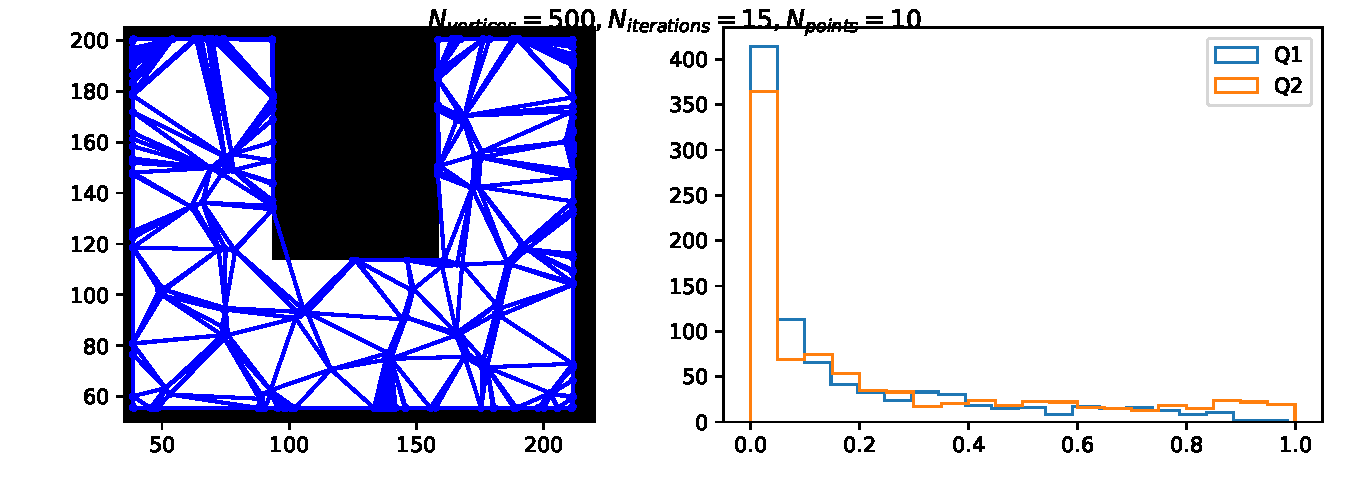
\includegraphics[width=\linewidth]{ex1.pdf}
	\caption{First attempt at generating a mesh. It went poorly}
	\label{fig:ex1}
\end{figure}

\begin{figure}
	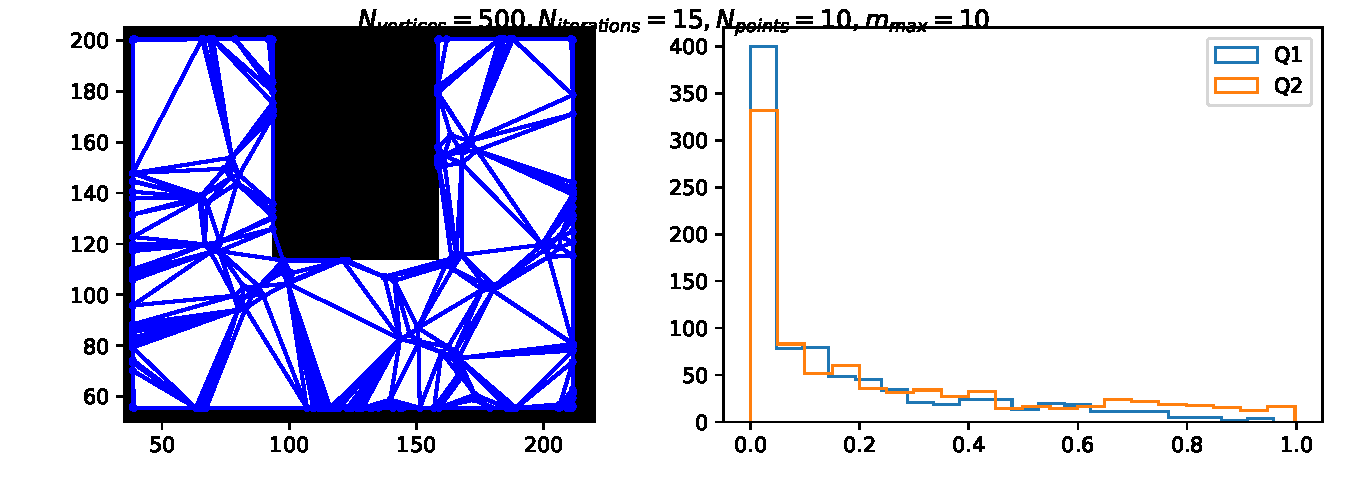
\includegraphics[width=\linewidth]{ex2.pdf}
	\caption{Second attempt at generating a mesh. Looks even worse}
	\label{fig:ex2}
\end{figure}
Both meshes are terrible. The majority of triangles fall into the first bin of the quality measures. If we instead use the \texttt{Triangle} package we get the result seen in figure \ref{fig:ex5}
\begin{figure}
	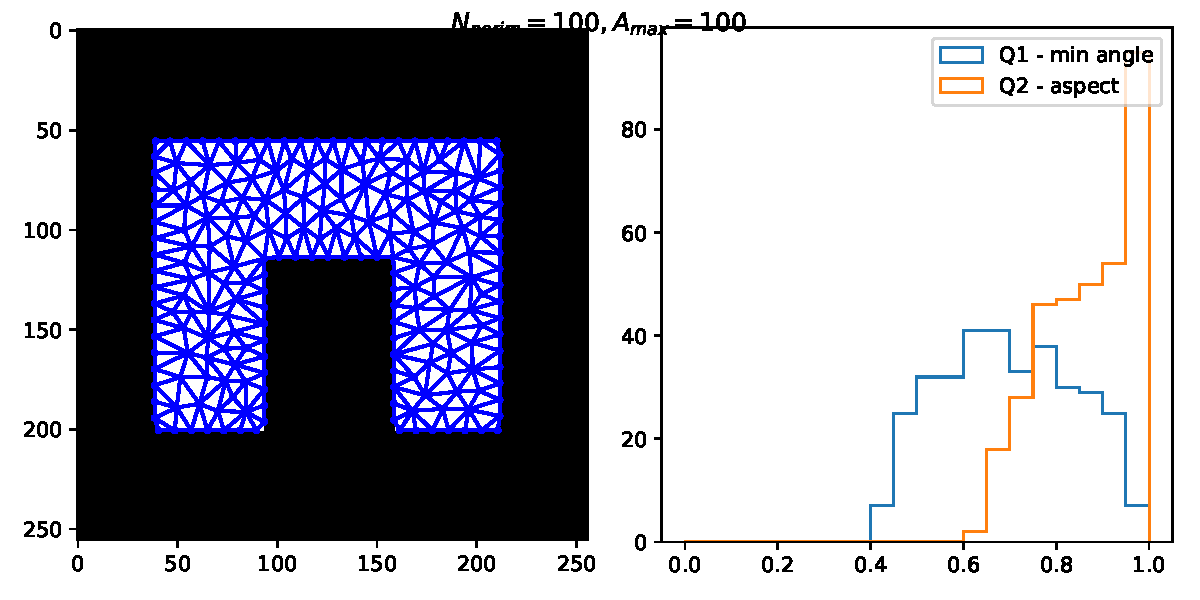
\includegraphics[width=\linewidth]{ex5.pdf}
	\caption{Creating a mesh from the sample image, there are 100 points along the border, and a max triangle area of 100 pixels}
	\label{fig:ex5}
\end{figure}
If we instead use the sample image from this week, we get the results seen in figures \ref{fig:ex4} and \ref{fig:ex3}. Again \texttt{Triangle} provides a much better mesh, especially compared to the ones created from scratch.
\begin{figure}
	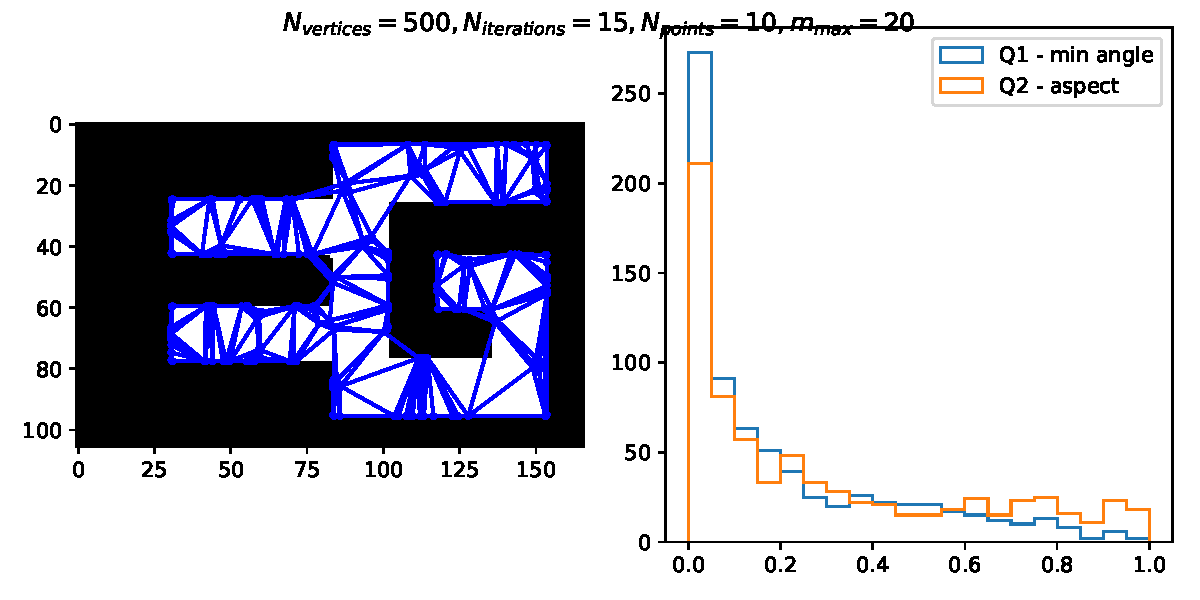
\includegraphics[width=\linewidth]{ex4.pdf}
	\caption{Creating a mesh with \texttt{Triangle}, from this weeks sample image. 200 vertices around the border, max area of 50.}
	\label{fig:ex4}
\end{figure}

\begin{figure}
	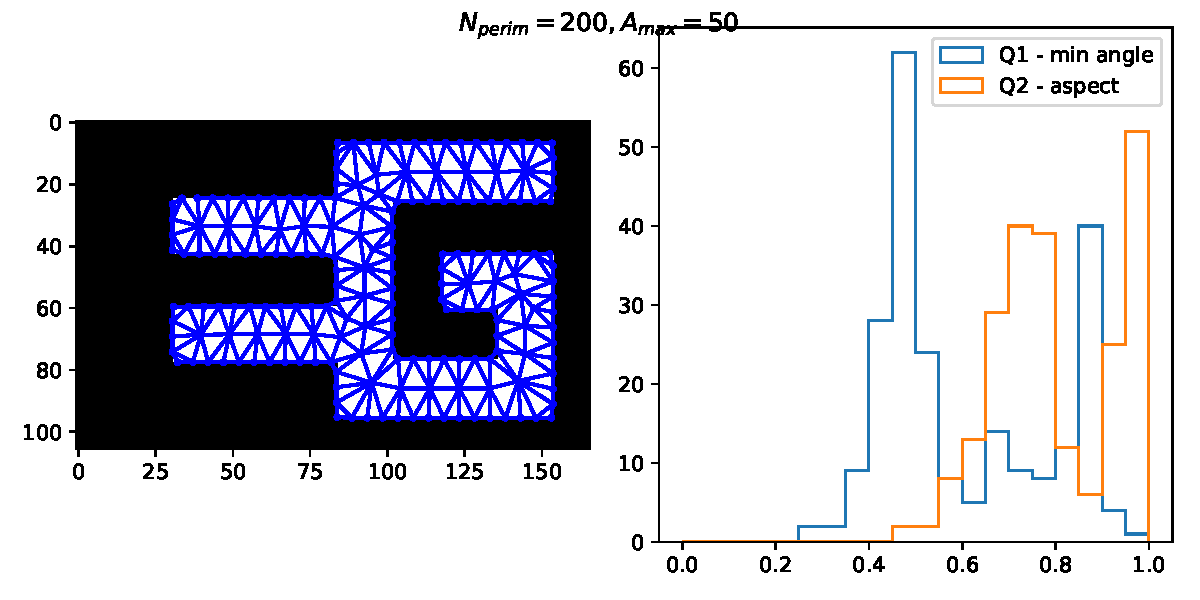
\includegraphics[width=\linewidth]{ex3.pdf}
	\caption{This weeks sample image, mesh created from scratch, 1000 vertices.}
	\label{fig:ex3}
\end{figure}
Lastly we look at an image with 3 separate geometries, with results in figures \ref{fig:ex7} and \ref{fig:ex6}.
\begin{figure}
	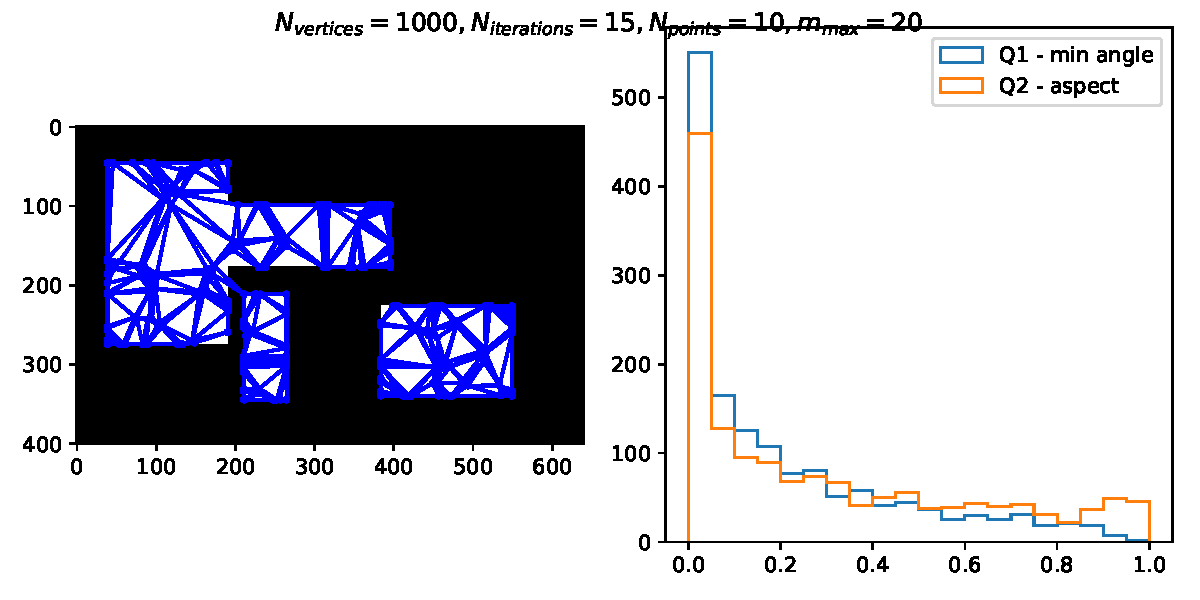
\includegraphics[width=\linewidth]{ex7.pdf}
	\caption{Mesh from scratch, for image with 3 separate geometries. 1000 vertices}
	\label{fig:ex7}
\end{figure}

\begin{figure}
	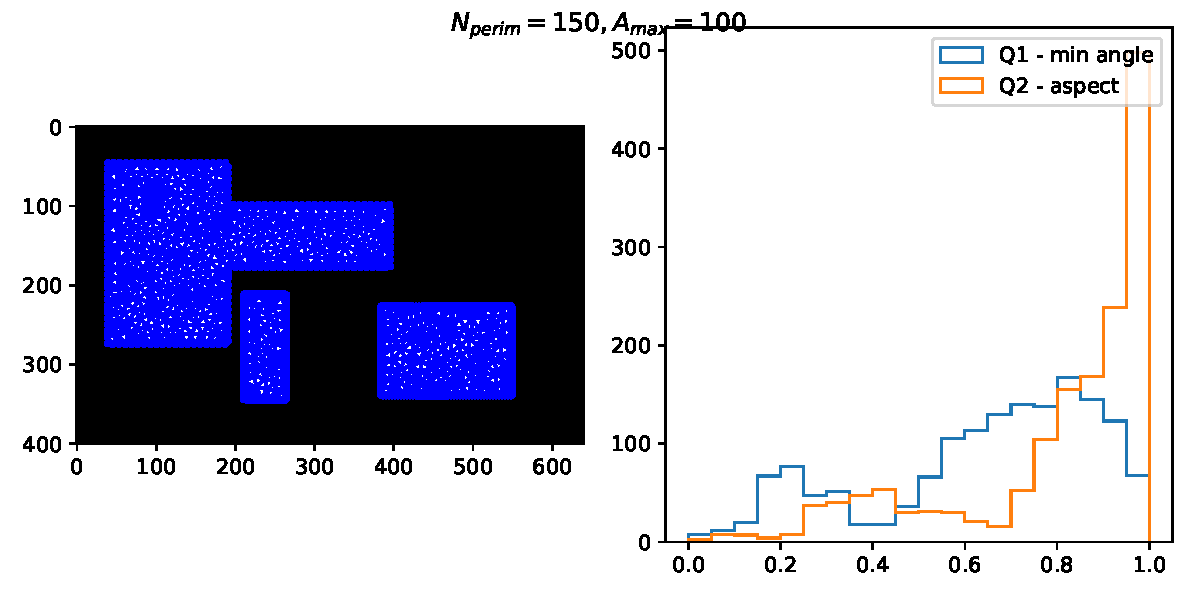
\includegraphics[width=\linewidth]{ex6.pdf}
	\caption{Mesh from \texttt{Triangle}, for image with 3 separate geometries. 100 points per contour, 100 max area}
	\label{fig:ex6}
\end{figure}
Note the drop in quality for the mesh generated from \texttt{Triangle}. This is due to the chosen parameters (100 points per contour). This fits fine for the larger geometries, but for the small rectangle, it is far too many, leading to a large number of triangles with far too shallow a minimum angle. Expanding the code to be able to handle different numbers of vertices per contour would alleviate the problem.

In conclusion we see that with the current implemented algorithm, the meshes generated from scratch are no where near an acceptable level of quality, whilst the meshes generated from \texttt{Triangle} perform much better. 

It is also worth noting the difference in distributions for the two quality measures. The minimum angle measure tends to have a much wider peak, at a lower value than that for the aspect ratio measure.


\end{document}
